\documentclass[12pt]{article}
\usepackage{amssymb}
\usepackage[cmex10]{amsmath}
\usepackage{verbatim}
\usepackage{courier}
\usepackage[T1]{fontenc}
\usepackage[margin=1in]{geometry}
\usepackage{setspace}
\usepackage{graphicx}
\singlespacing
\setlength{\parindent}{0pt}

\begin{document}

%%%%%%%%%%%%%%%%%%%%%%%%%%%%%%%%%%%%%%%%%%%%%%%%%%%%%%%%%%%%%%%%%%%%%%%%%%%%%%%%%%%%%%

\section*{Imaginary Numbers}
An imaginary number $a+jb$, has magnitude $M = \sqrt{a^2+b^2}$, and phase $\phi = \tan^{-1}(b/a)$\\

\begin{center}
	$a+jb = Me^{-j\phi} = M\angle\phi $
\end{center}
Where $j = i = \sqrt{-1}$

%%%%%%%%%%%%%%%%%%%%%%%%%%%%%%%%%%%%%%%%%%%%%%%%%%%%%%%%%%%%%%%%%%%%%%%%%%%%%%%%%%%%%%

\section*{KVL/KCL}
KVL $\rightarrow$ The sum of all voltages in a loop must be zero. \\
KCL $\rightarrow$ The sum of currents in and out of a node must be zero. \\

\begin{center}
	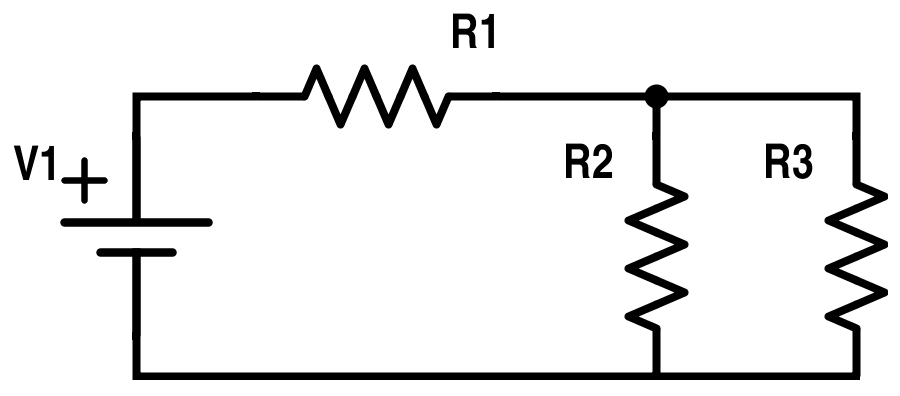
\includegraphics[width=0.8\textwidth]{assets/ece210-kvl.png}
\end{center}

KVL example, using ``positive voltage'' as $+\rightarrow-$:
\begin{center}
	$-V_1 + V_{R1} + V_{R2} = 0$\\
	$-V_1 + V_{R1} + V_{R3} = 0$\\
	$-V_{R2} + V_{R3} = 0$
\end{center}

KCL example, using the node where the resistors meet:
\begin{center}
	$i_{R1} = i_{R2} + i_{R3}$
\end{center}


%%%%%%%%%%%%%%%%%%%%%%%%%%%%%%%%%%%%%%%%%%%%%%%%%%%%%%%%%%%%%%%%%%%%%%%%%%%%%%%%%%%%%%

\section*{Impedance}
Resistors have real resistance $R = V/I$, measured in Ohms ($\Omega$)\\
Resistors in series add cumulatively: $R_{ser} = R_1+R_2$\\
Resistors in parallel add inversely:  $1/R_{par} = 1/R_1 + 1/R_2$, or $R_{par} = \dfrac{R_1R_2}{R_1+R_2}$\\

\newpage

Capacitors have imaginary reactance $I = C \dfrac{\partial V}{\partial t}$, or $Z_c = 1/j\omega C$, measure in Farads (F)\\
Capacitors in series add inversely: $1/C_{ser} = 1/C_1 + 1/C_2$, or $C_{ser} = \dfrac{C_1C_2}{C_1+C_2}$\\
Capacitors in parallel add cumulatively: $C_{par} = C_1 + C_2$\\

Inductors have imaginary reactance $V = L \dfrac{\partial i}{\partial t}$, measured in Henries (H)\\
Inductors in series add cumulatively: $L_{ser} = L_1 + L_2$\\
Inductors in parallel add inversely: $1/L_{par} = 1/L_1 + 1/L_2$, or $L_{par} = \dfrac{L_1L_2}{L_1+L_2}$\\

%%%%%%%%%%%%%%%%%%%%%%%%%%%%%%%%%%%%%%%%%%%%%%%%%%%%%%%%%%%%%%%%%%%%%%%%%%%%%%%%%%%%%%

\section*{Time Domain RLC}

Important constants $100\%*e^{-1} = 36\%$ and  $100\%*(1-e^{-1}) = 63\%$ \\

\begin{center}
	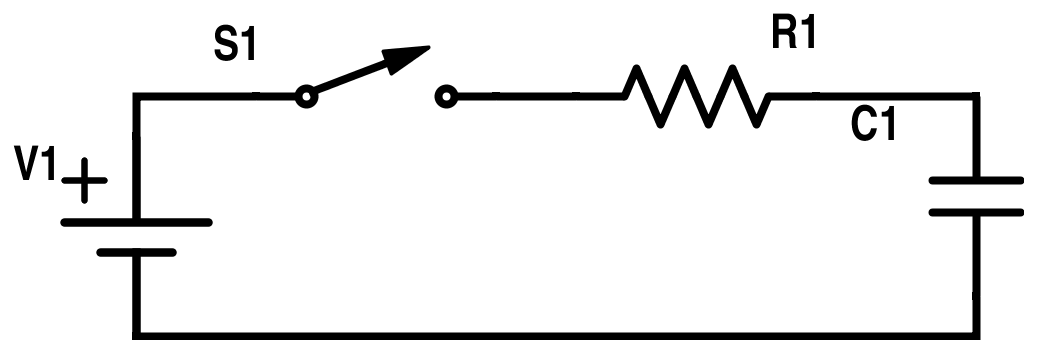
\includegraphics[width=0.8\textwidth]{assets/ece210-rc.png}
\end{center}

RC Circuits have a time constant $\tau = RC$, and are exponential functions\\
Discharging capacitors decay at a rate of $V(t) = V_0 e^{-t/\tau}$\\
Charging capacitors charge at a rate of $V(t) = V_0 (1 - e^{-t/\tau})$\\

RL Circuits have a time constant $\tau = R/L$, and are exponential functions\\

LC Circuits have a time constant $\tau = 1/\sqrt{LC}$, and are sinusoidal functions\\

RLC Circuits have time constant $\tau =  1/\sqrt{LC}$, and are dampened sinusoidal functions

%%%%%%%%%%%%%%%%%%%%%%%%%%%%%%%%%%%%%%%%%%%%%%%%%%%%%%%%%%%%%%%%%%%%%%%%%%%%%%%%%%%%%%

\section*{Power}

Passing current through a resistor consumes power. Capacitors and inductors store energy, but do not dissipate power. The instantaneous power burned by a resistor is:
\[ P_{inst} = V\cdot I = \dfrac{V^2}{R} = \dfrac{I^2}{R} \]

We can also define average power of some periodic waveform: 
\[ P = \dfrac{1}{T} \int_{t=0}^T v(t)i(t)dt = \dfrac{1}{2}\mathrm{Re}\{VI^*\} \]

It's easier to see this with a sine wave and RMS values ($V_{pk} = \sqrt{2}V_{rms})$:

\[ P = \dfrac{{V_{rms}}^2}{R} = \left(\dfrac{V_{pk}}{\sqrt{2}}\right)^2\dfrac{1}{R} = \dfrac{{V_{pk}}^2}{2R} \]

Another important metric is available power, or how much power can a source with some resistance deliver to a load.

\begin{center}
	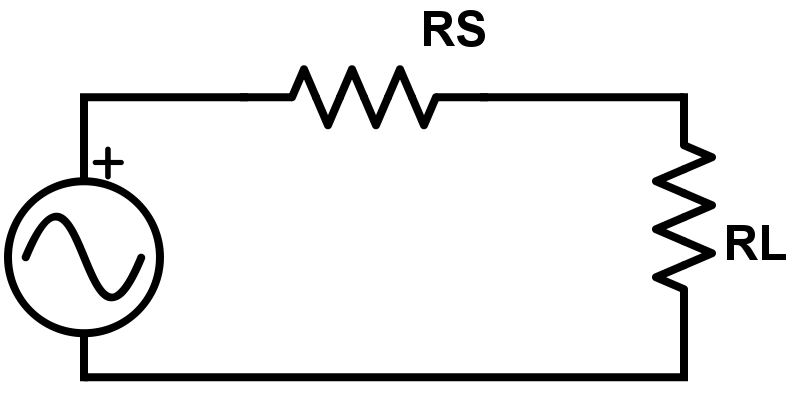
\includegraphics[width=0.8\textwidth]{assets/ece210-power-available.png}
\end{center}

We can prove that the maximum power is delivered to the load when $R_S = R_L$. When the resistance is equal, each resistor sees half the voltage, so the maximum power that the load resistor can use is:

\[P_a = \left(\dfrac{V_{rms}}{2}\right)^2 \dfrac{1}{R_L} = \dfrac{V_{rms}}{4R_L} = \dfrac{V_{pk}}{8R_L} \]
%%%%%%%%%%%%%%%%%%%%%%%%%%%%%%%%%%%%%%%%%%%%%%%%%%%%%%%%%%%%%%%%%%%%%%%%%%%%%%%%%%%%%%

\section*{Fourier/Transfer Function}

We use Fourier transforms to go from time to frequency domain. Some time domain signal $f(t)$ can represented in the frequency domain as $F(w)$ through:

\[ F(w) = \int_{-\infty}^{\infty} f(t)e^{jwt}dw \]

These are pretty ugly math expressions in general, so only a few are worth memorizing:

\[ \cos(w_0t) \leftrightarrow \pi[\delta(w-w_0) + \delta(w+w_0)]\] 
\[ \dfrac{df(t)}{dt} \leftrightarrow  jwF(w)\]
\[ x(t)*h(t) \leftrightarrow X(w)H(w) \]

This helps us represent circuits in another way: transfer functions. These are defined by their magnitude and phase. We noramlly draw them on a log-log (log-dB) scale. The two classical ones are high pass and low pass filters.  \\

High pass filters have a magnitude of 1 as $w\rightarrow\infty$, and take the form:
\[H(w) = \dfrac{jw}{1+jw}\]
\begin{center}
	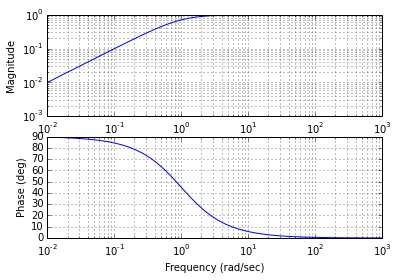
\includegraphics[scale=0.75]{assets/ece210-hpf.png}
\end{center}

Low pass filters have a magnitude of 1 as $w \rightarrow 0$, and take the form:
\[H(w) = \dfrac{1}{1+jw}\]
\begin{center}
	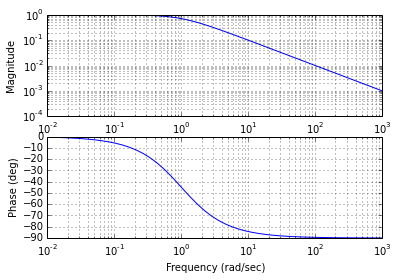
\includegraphics[scale=0.75]{assets/ece210-lpf.png}
\end{center}

%%%%%%%%%%%%%%%%%%%%%%%%%%%%%%%%%%%%%%%%%%%%%%%%%%%%%%%%%%%%%%%%%%%%%%%%%%%%%%%%%%%%%%

\section*{Frequency Domain RLC}
Sometimes it's simpler to represent RLC circuits in frequency domain rather than time domain. We can now define each RLC element as an impedance $Z$:
\begin{itemize}
	\item $Z_R = R$
	\item $Z_C = \dfrac{1}{jwC}$
	\item $Z_L = jwL$
\end{itemize}

This modifies Ohm's Law to be $V = I Z$. We treat impedances like resistors, summing them cumulatively in series, and inversely in parallel. 

%%%%%%%%%%%%%%%%%%%%%%%%%%%%%%%%%%%%%%%%%%%%%%%%%%%%%%%%%%%%%%%%%%%%%%%%%%%%%%%%%%%%%%

\section*{Op Amps}
Op amps are a common active component in EE. They have five terminals:
\begin{enumerate}
	\item Positive Input
	\item Negative Input
	\item Output
	\item Positive Supply
	\item Negative Supply
\end{enumerate}

\begin{center}
	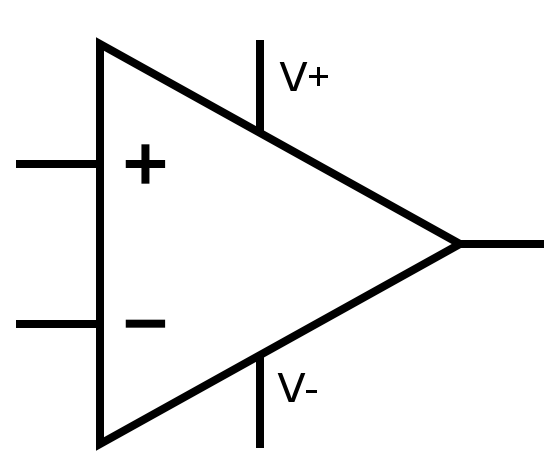
\includegraphics[height=1in]{assets/ece210-opamp5.png}
\end{center}

While they are complex devices, we can abstract them with three rules:

\begin{itemize}
	\item No current flows into the positive/negative inputs
	\item The voltage at the positive/negative inputs is the same
	\item The output voltage can't go above or below the supply
\end{itemize}

\begin{center}
	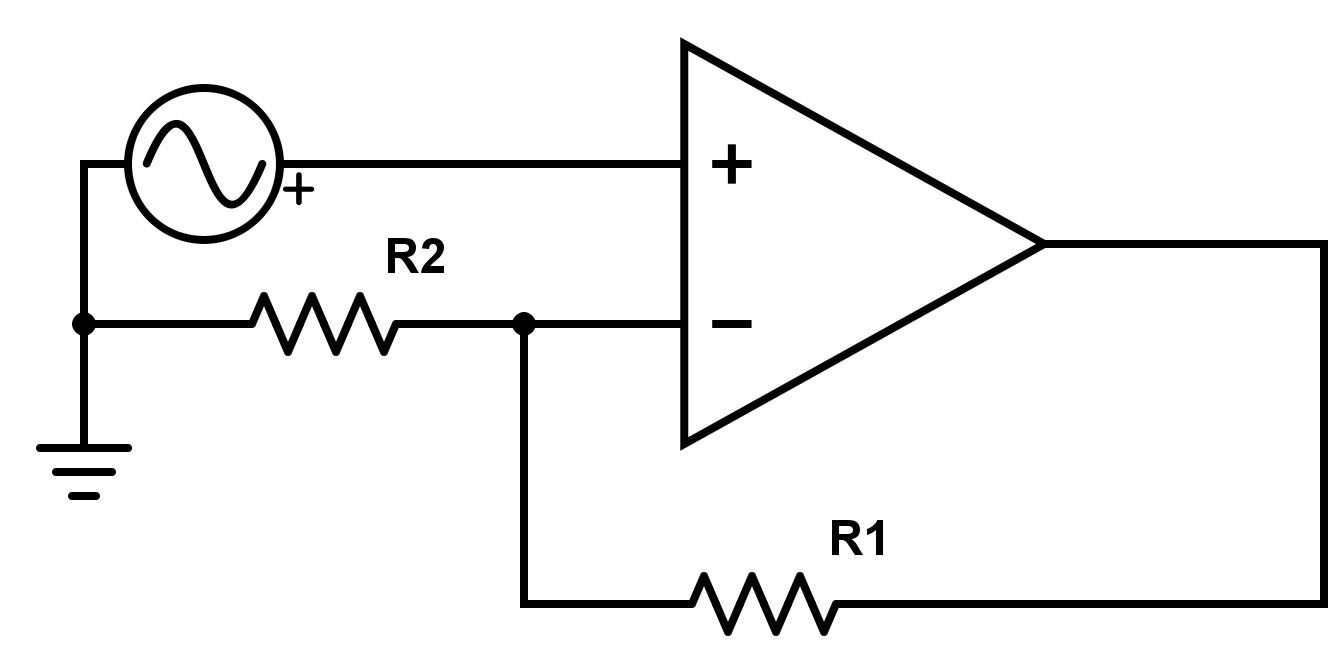
\includegraphics[height=2in]{assets/ece210-opamp-circuit.png}
\end{center}

As an example of how to solve this circuit:
\[ V_+  = V_{in} = V_- \]
\[ i_{R2} = \dfrac{Vin}{R2} = i_{R1} \]
\[ V_{out} - V_- = i_{R1} R_1 \]
\[ V_{out} = V_{in} + V_{in}\dfrac{R1}{R2} \]
\[ V_{out} = V_{in} \left( 1 + \dfrac{R1}{R2} \right) \]
%%%%%%%%%%%%%%%%%%%%%%%%%%%%%%%%%%%%%%%%%%%%%%%%%%%%%%%%%%%%%%%%%%%%%%%%%%%%%%%%%%%%%%

% \section*{AM Radio/Mixing}
% TBD?

% SYLLABUS FROM WEBSITE
\begin{comment}
	This list comes from the ECE210 syllabus:
	Examples of signals and signal processing systems
	Analog linear time-invariant systems
	Circuits and linear systems
	Review of DC circuit analysis: KCL, KVL, dependent sources
	Capacitors and inductors as circuit elements
	Op-amp circuits
	Characterization and solution of LSI systems via linear, constant-coefficient differential equations
	Complex numbers and functions of a complex variable
	Impedance, phasors, and sinusoidal steady-state
	Frequency response and multi-frequency circuits
	Fourier Series
	Fourier transform
	AM radio
	Convolution
	Impulse and impulse response
	Sampling theorem and overview of digital signal processing
	Stability
	Laplace transform and transfer function
	Laplace transform solution of differential equations
	General form of solution to a differential equation
	Design of active filters
\end{comment}

\end{document}